\chapter{Unit Tests}
\label{app:unittest}


\section{Visual Studio Test Viewer}
\begin{figure}[H]
    \centering
    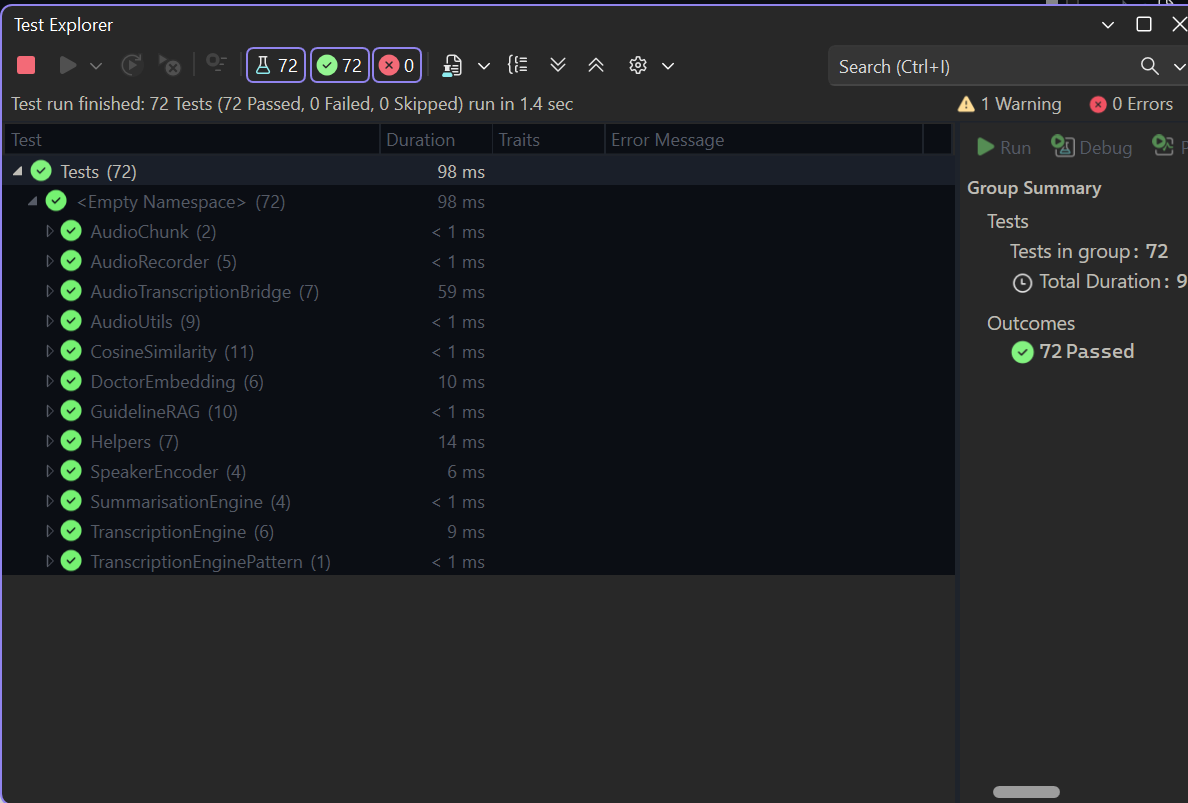
\includegraphics[width=0.5\linewidth]{unittest.png}
    \caption{All 72 unit tests passing in the Visual Studio Test Viewer}
    \label{fig:unittest_results}
\end{figure}

\section{Unit Test Cases}
\begingroup
\footnotesize % Reduces the font size for everything inside this group
\begin{longtable}{|p{0.32\textwidth}|p{0.53\textwidth}|c|}
\hline
\textbf{Test Name} & \textbf{Description} & \textbf{Pass} \\
\hline
\endfirsthead

\hline
\textbf{Test Name} & \textbf{Description} & \textbf{Pass} \\
\hline
\endhead

% --- AudioRecorder ---
\hline
\multicolumn{3}{|c|}{\textbf{AudioRecorder}} \\
\hline
DelegatesStartToBackend & Verifies audio recorder delegates Start to injected backend. & Yes \\ \hline
DelegatesStopToBackend & Verifies audio recorder delegates Stop to injected backend. & Yes \\ \hline
DelegatesStartMultipleTimes & Verifies backend start can be called multiple times. & Yes \\ \hline
DelegatesStopWithoutStart & Verifies backend stop can be called safely without a prior start. & Yes \\ \hline
DelegatesStartThenStop & Verifies start and stop both route through seam on same instance. & Yes \\ \hline

% --- AudioTranscriptionBridge ---
\hline
\multicolumn{3}{|c|}{\textbf{AudioTranscriptionBridge}} \\
\hline
PushAndPopSingleChunk & Verifies single chunk roundtrip. & Yes \\ \hline
FIFOOrdering & Verifies FIFO ordering. & Yes \\ \hline
PopBlocksUntilPush & Verifies blocking pop. & Yes \\ \hline
EmptyAudioDataChunk & Verifies empty payload handling. & Yes \\ \hline
PreservesIsLastFalse & Verifies false isLast flag is preserved through queueing. & Yes \\ \hline
PreservesOrderAndLastMarker & Verifies two-chunk order and final marker are preserved. & Yes \\ \hline
PopsPreBufferedItems & Verifies pop can consume pre-buffered multiple items without blocking. & Yes \\ \hline
ConcurrentProducersComplete & Verifies concurrent producers preserve total item count. & Yes \\ \hline

% --- AudioUtils ---
\hline
\multicolumn{3}{|c|}{\textbf{AudioUtils}} \\
\hline
NormaliseScalesMidAmplitude & Verifies scaling path. & Yes \\ \hline
NormaliseSkipsQuietAudio & Verifies quiet threshold path. & Yes \\ \hline
NormaliseSkipsAlreadyLoudAudio & Verifies loud threshold path. & Yes \\ \hline
NormaliseSkipsLowerBoundary & Verifies lower boundary max\_amp==0.001 is not scaled. & Yes \\ \hline
NormaliseSkipsUpperBoundary & Verifies upper boundary max\_amp==0.9 is not scaled. & Yes \\ \hline
NormalisePreservesSigns & Verifies normalization keeps sample signs intact. & Yes \\ \hline
NormaliseHandlesEmptyBuffer & Verifies empty audio buffers are handled safely. & Yes \\ \hline
NormaliseSingleSample & Verifies single sample normalization reaches target amplitude. & Yes \\ \hline
NormaliseAllZerosNoChange & Verifies normalization keeps zeros unchanged. & Yes \\ \hline

% --- CosineSimilarity ---
\hline
\multicolumn{3}{|c|}{\textbf{CosineSimilarity}} \\
\hline
IdenticalVectors & Verifies cosine=1 for identical vectors. & Yes \\ \hline
OrthogonalVectors & Verifies orthogonal vectors. & Yes \\ \hline
OppositeVectors & Verifies opposite vectors. & Yes \\ \hline
DifferentSizesReturnZero & Verifies mismatch branch. & Yes \\ \hline
EmptyVectorsReturnZero & Verifies empty branch. & Yes \\ \hline
ZeroVectorReturnZero & Verifies zero denominator branch. & Yes \\ \hline
ScaledDirection & Verifies scale invariance. & Yes \\ \hline
SymmetricResult & Verifies cosine similarity is symmetric. & Yes \\ \hline
OneDimensionalPositive & Verifies one-dimensional positive vectors return full similarity. & Yes \\ \hline
OneDimensionalOpposite & Verifies one-dimensional opposite vectors return negative similarity. & Yes \\ \hline
MixedSignsWithinBounds & Verifies mixed sign vectors produce bounded similarity. & Yes \\ \hline

% --- DoctorEmbedding ---
\hline
\multicolumn{3}{|c|}{\textbf{DoctorEmbedding}} \\
\hline
SetStorageDirectoryAndProfileFlagPath & Verifies doctor embedding stores override directory. & Yes \\ \hline
DelegatesEnrollAndSaveToBackend & Verifies doctor embedding delegates enrollment capture and save to injected backend. & Yes \\ \hline
DelegatesLoadToBackend & Verifies doctor embedding delegates load path through backend when memory cache is empty. & Yes \\ \hline
EmptyCapturedAudioSkipsSave & Verifies enrollment with empty captured audio does not save profile. & Yes \\ \hline
LoadFromBackendIsCached & Verifies loading from backend is cached after first fetch. & Yes \\ \hline
UsesBackendDefaultPathForSave & Verifies backend default path is used when no storage override is set. & Yes \\ \hline

% --- GuidelineRAG ---
\hline
\multicolumn{3}{|c|}{\textbf{GuidelineRAG}} \\
\hline
UsesInjectedBackendForInitialize & Verifies initialize delegation through interface seam. & Yes \\ \hline
UsesInjectedBackendForEmbedText & Verifies embed delegation through seam. & Yes \\ \hline
UsesInjectedBackendForQuery & Verifies query delegation through seam. & Yes \\ \hline
UsesInjectedBackendForReload & Verifies reload delegation through seam. & Yes \\ \hline
UsesInjectedBackendForHasIndex & Verifies has-index delegation through seam. & Yes \\ \hline
QueryReturnsEmptyWhenNoBackend... & Verifies null-impl safe path. & Yes \\ \hline
QueryForwardsInputAndTopK & Verifies query text and topK are forwarded to injected backend. & Yes \\ \hline
EmbedTextForwardsInput & Verifies embed text is forwarded to injected backend. & Yes \\ \hline
QueryUsesDefaultTopKWhenOmitted & Verifies default topK value is forwarded when omitted. & Yes \\ \hline
HasIndexFalseFromBackend & Verifies backend false index state is reflected by wrapper. & Yes \\ \hline
HasIndexReflectsBackendToggle & Verifies backend true index state can be toggled after injection. & Yes \\ \hline

% --- Helpers ---
\hline
\multicolumn{3}{|c|}{\textbf{Helpers}} \\
\hline
GetModelPathWithOverride & Verifies override path usage. & Yes \\ \hline
GetModelPathSubfolder & Verifies slash normalization. & Yes \\ \hline
GetGuidelinesDataPathCreatesFolder & Verifies directory creation branch. & Yes \\ \hline
OverrideCanBeCleared & Verifies clear override behavior. & Yes \\ \hline
GetGuidelinesDataPathStable... & Verifies same override returns same data folder path each call. & Yes \\ \hline
GetModelPathNestedSegments & Verifies nested model path joining works. & Yes \\ \hline
GetGuidelinesDataPathSuffix & Verifies guidelines data path points to guidelines\_data suffix. & Yes \\ \hline

% --- AudioChunk ---
\hline
\multicolumn{3}{|c|}{\textbf{AudioChunk}} \\
\hline
DefaultIsNotLast & Verifies default isLastChunk value. & Yes \\ \hline
DefaultAudioIsEmpty & Verifies default audio vector empty. & Yes \\ \hline
AudioDataCanBeAssigned & Verifies chunk audio is mutable as expected. & Yes \\ \hline

% --- SpeakerEncoder ---
\hline
\multicolumn{3}{|c|}{\textbf{SpeakerEncoder}} \\
\hline
DelegatesInitializeToBackend & Verifies speaker encoder delegates initialization to injected backend. & Yes \\ \hline
DelegatesEmbeddingToBackend & Verifies speaker encoder delegates embedding to injected backend. & Yes \\ \hline
DelegatesEmptyEmbedding & Verifies encoder can return empty embeddings from backend. & Yes \\ \hline
RepeatedInitializeUpdatesArgs & Verifies repeated initialize calls update backend args. & Yes \\ \hline
EmbeddingCapturesSingleSampleInput & Verifies embedding input is captured exactly for boundary-size vectors. & Yes \\ \hline

% --- SummarisationEngine ---
\hline
\multicolumn{3}{|c|}{\textbf{SummarisationEngine}} \\
\hline
DelegatesLoadModelToBackend & Verifies summarisation load delegates model path to injected backend. & Yes \\ \hline
DelegatesGenerateToBackend & Verifies summarisation prompt and generation parameters are forwarded to backend. & Yes \\ \hline
HandlesEmptyBackendOutput & Verifies summarisation backend can return empty output. & Yes \\ \hline
ForwardsMultilineTranscript & Verifies multiline transcript is forwarded into prompt. & Yes \\ \hline
IncludesSystemPromptHeader & Verifies system prompt header is included. & Yes \\ \hline
IncludesAssistantMarker & Verifies assistant marker is included in composed prompt. & Yes \\ \hline
HandlesEmptyTranscriptInput & Verifies empty transcript still composes a valid prompt. & Yes \\ \hline

% --- TranscriptionEngine ---
\hline
\multicolumn{3}{|c|}{\textbf{TranscriptionEngine}} \\
\hline
CancelDuringLoopReturnsEmpty & Verifies cancellation while loop is waiting returns empty transcript. & Yes \\ \hline
LabelsDoctorWithHighSimilarity & Verifies transcription engine labels a long segment as doctor when similarity is high. & Yes \\ \hline
LabelsPatientWithLowSimilarity & Verifies transcription engine labels a long segment as patient when similarity is low. & Yes \\ \hline
KeepsUnknownForShortSegments & Verifies transcription engine keeps unknown label for short segments. & Yes \\ \hline
InitialiseModelDelegatesPath & Verifies transcription backend model initialization path is passed through. & Yes \\ \hline
AppendsMultipleChunks & Verifies multiple generated chunks are appended into transcript. & Yes \\ \hline
IsCancelledReflectsState & Verifies cancellation flag accessor reflects cancellation calls. & Yes \\ \hline
GenerateCalledForInputChunk & Verifies generated chunks function is invoked once per input chunk. & Yes \\ \hline
OutOfRangeTimestampsAreClamped & Verifies out-of-range timestamps do not crash and still produce output line. & Yes \\ \hline
\end{longtable}
\endgroup